\subsection{Описание клиентской библиотеки}
Клиентская библиотека --- программный модуль в составе сервиса управления виртуализированной инфраструктурой, который отвечает за взаимодействие с каждой из поддерживаемых платформ облачных вычислений, а так же предоставляет унифицированный программный интерфейс (API), не зависящий от конкретной платформы.

На рис.~\ref{lib-classes} приведена диаграмма классов клиентской библиотеки.
В центре диаграммы находятся два интерфейса ''AppClient'' и ''AppInstance'', которые служат для абстрагирования пользователей библиотеки от такого с какой именно платформой облачных вычислений они работают.

\begin{figure}[hbtp]
    \centering
    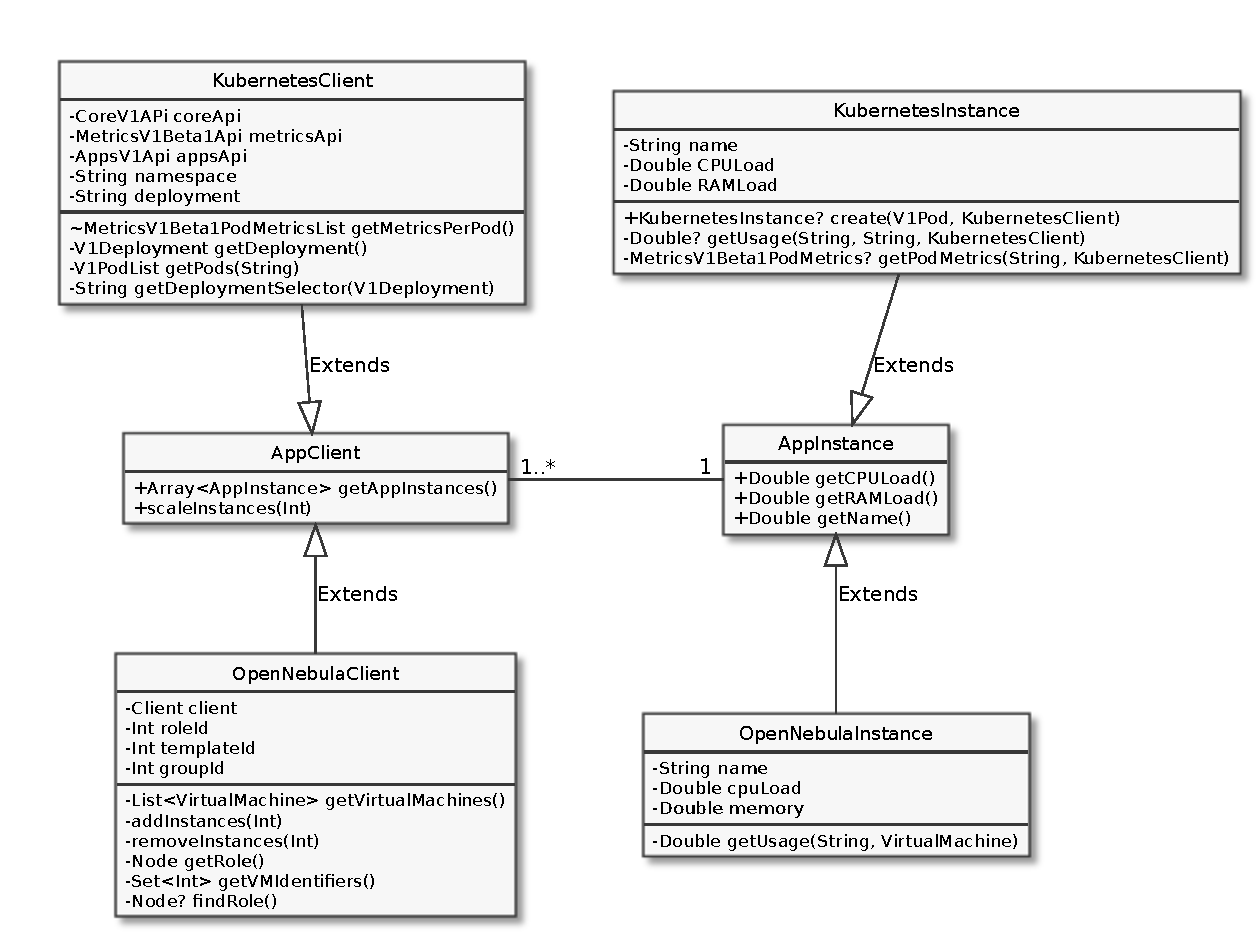
\includegraphics[width=\textwidth]{img/lib-classes.pdf}
    \caption{Диаграмма классов}
    \label{lib-classes}
\end{figure}

В частности, ''AppClient'' предоставляет интерфейс взаимодействия с приложением, а именно два метода:
\begin{enumerate}
    \item getAppInstances --- метод для получения списка ВМ или контейнеров, выделенных этому приложению;
    \item scaleInstances --- метод для изменения количества выделенных приложению ВМ или контейнеров.
\end{enumerate}

Выделенные приложению ВМ или контейнеры (в зависимости от платформы) представлены интерфейсом ''AppInstance'', который позволяет узнать своё имя, заданное на платформе облачных вычислений, а так же собранную статистическую информацию по использованным ресурсам.
В частности, ''getCPULoad'' возвращает загрузку вычислительных ядер в течение последней минуты, а ''getRAMLoad'' возвращает количество используемых приложением байт оперативной памяти.

Остальные классы на данной диаграмме являются реализациями двух описанных выше интерфейсов под конкретные виртуализированные инфраструктуры.
Как видно из набора полей и методов этих классов, внутренне они существенно различаются, но, несмотря на это, пользователи библиотеки могут взаимодействовать с ними через один и тот же интерфейс, что ускоряет и упрощает разработку новых модулей облачных систем.

\FloatBarrier